\documentclass[11pt,a4paper]{article}
\usepackage[margin=2cm]{geometry}
\usepackage[T1]{fontenc}
\usepackage{graphicx}
\usepackage[table]{xcolor}
\usepackage{booktabs}
\usepackage{array}
\usepackage{float}
\usepackage{fancyhdr}
\usepackage{hyperref}
\usepackage{titlesec}
\usepackage{caption}

\definecolor{labgreen}{HTML}{2F7456}
\definecolor{lightgreen}{HTML}{EAF3EE}
\hypersetup{colorlinks=true,urlcolor=labgreen,linkcolor=labgreen}
\titleformat{\section}{\Large\bfseries\color{labgreen}}{\thesection}{0.6em}{}
\titleformat{\subsection}{\large\bfseries\color{labgreen}}{\thesubsection}{0.6em}{}
\pagestyle{fancy}
\fancyhf{}
\lhead{\small LAB 02 \quad Robot Vision}
\cfoot{\small Stereo Depth Estimation Report \quad | \quad \thepage}
\renewcommand{\headrulewidth}{0pt}
\setlength{\parindent}{2em}
\setlength{\parskip}{0.35em}

\begin{document}

{\large\bfseries\color{labgreen} LAB REPORT / ROBOT VISION\par}
\vspace{0.5em}
{\LARGE\bfseries Stereo Depth Estimation Using OpenCV\par}
\vspace{0.3em}
{\large\color{gray} Based on the OpenCV Aloe Stereo Pair and StereoSGBM\par}
\vspace{1.2em}

\renewcommand{\arraystretch}{1.45}
\begin{tabular}{>{\columncolor{lightgreen}\bfseries}p{2cm}p{4.6cm}>{\columncolor{lightgreen}\bfseries}p{2.4cm}p{4.2cm}}
Name & Zhang Linjie & Student ID & 24020036086 \\
Date & September 25, 2026 & Course & Robot Vision \\
\end{tabular}

\section{Experiment Overview}
This experiment implements binocular disparity estimation and relative-depth visualization with OpenCV. The official OpenCV aloe stereo pair is used as input. StereoSGBM matches corresponding pixels, and the fixed-point output is converted to pixel disparity for visualization.

The execution completed successfully on images of $1282 \times 1110$ pixels. The positive-disparity ratio was 78.07\%. It expresses the coverage of usable disparity rather than an accuracy measurement.

\begin{table}[H]
\centering
\rowcolors{2}{lightgreen}{white}
\begin{tabular}{cccc}
\rowcolor{labgreen}\color{white}\bfseries Stereo Pair & \color{white}\bfseries Image Size & \color{white}\bfseries Valid Disparity & \color{white}\bfseries Conclusion \\
AloeL / AloeR & $1282 \times 1110$ px & 78.07\% & Successful \\
\end{tabular}
\end{table}

\section{Principle of Stereo Depth Estimation}
After stereo rectification, corresponding points lie on the same horizontal line. Their horizontal displacement is disparity $d$. With focal length $f$ and baseline $B$, metric depth is $Z=fB/d$. Nearby objects therefore have larger disparity, while distant objects have smaller disparity.

The supplied pair is suitable for matching, but calibrated focal length and baseline are not used here. The program therefore displays relative depth $1/d$ rather than distance in metres. Zero or negative disparity is invalid and is displayed in black.

\section{Experimental Environment and Parameters}
\begin{table}[H]
\centering
\rowcolors{2}{lightgreen}{white}
\begin{tabular}{p{5cm}p{8cm}}
\rowcolor{labgreen}\color{white}\bfseries Item & \color{white}\bfseries Configuration \\
Programming Language & Python 3.8 \\
Vision Library & OpenCV 4.12.0 \\
Numerical Library & NumPy 1.24.4 \\
Input Images & OpenCV \texttt{aloeL.jpg} and \texttt{aloeR.jpg} \\
Stereo Method & StereoSGBM 3-way \\
Number of Disparities & 128 \\
Matching Block Size & $5 \times 5$ \\
\end{tabular}
\end{table}

\section{Experimental Method}
\subsection{Input Preparation}
The script \texttt{download\_opencv\_samples.py} downloads \texttt{aloeL.jpg} and \texttt{aloeR.jpg} from the official OpenCV sample-data repository into the \texttt{data/} directory. The images are two views of the same static scene and have identical dimensions.

\begin{figure}[H]
\centering
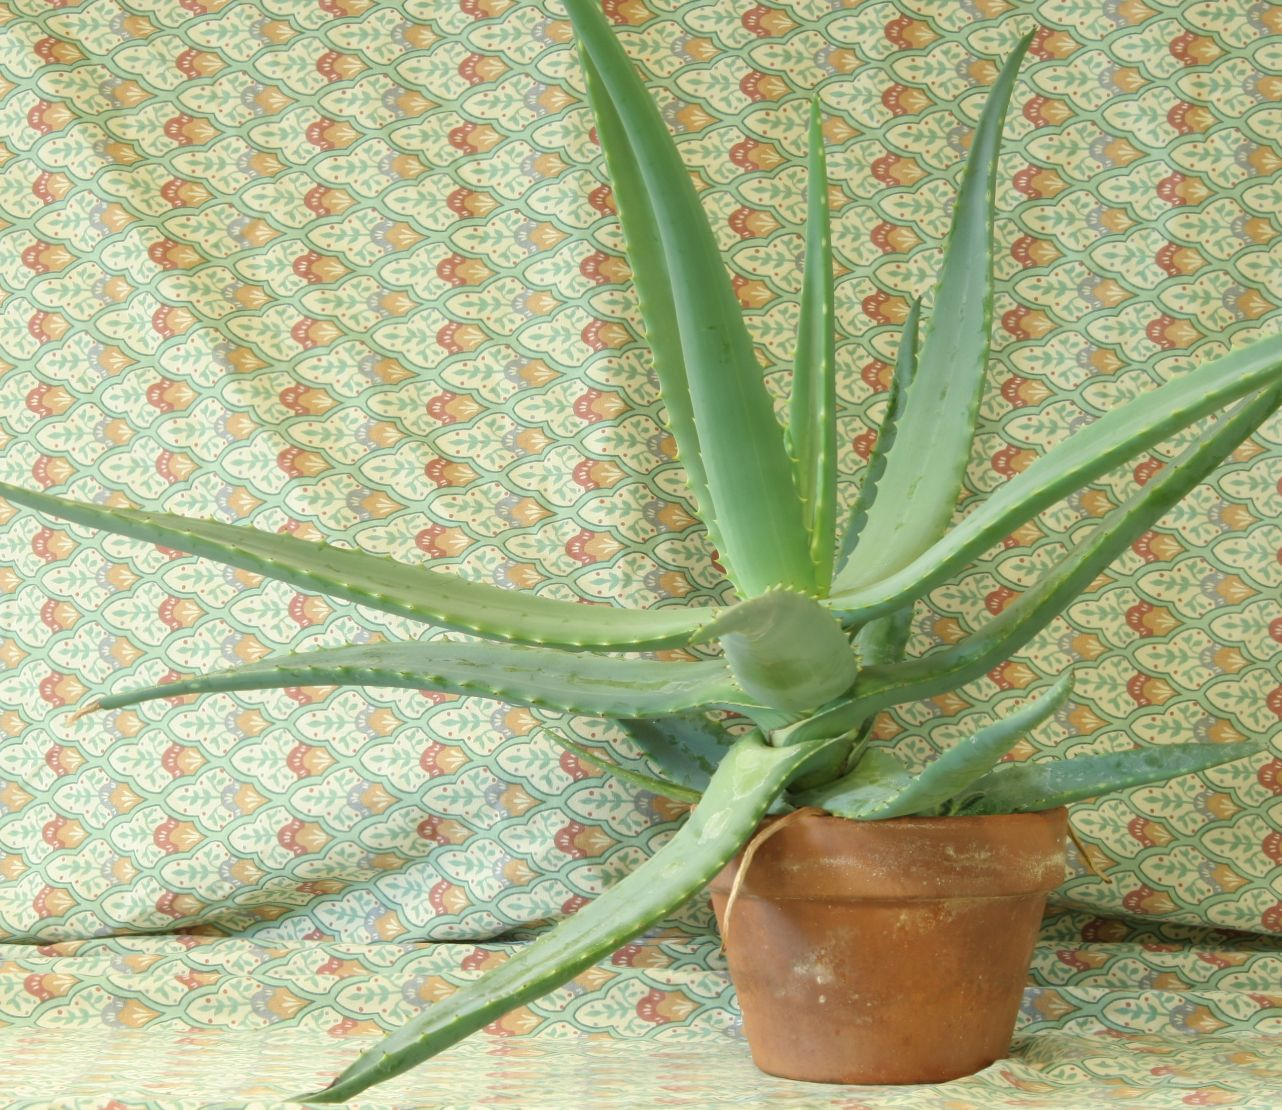
\includegraphics[width=0.68\textwidth]{../results/left.png}
\caption{Left image from the OpenCV aloe stereo pair.}
\end{figure}

\subsection{Disparity Computation}
Both images are converted to grayscale. StereoSGBM uses 128 disparities, a $5 \times 5$ matching window, uniqueness filtering, and speckle filtering. The returned fixed-point disparity is divided by 16.0 to obtain pixel disparity.

\subsection{Relative-depth Visualization}
For valid pixels, relative depth is computed as $1/d$. The 2nd and 98th percentiles normalize the displayed range. A TURBO colour map makes changes in disparity and relative depth easier to inspect.

\begin{center}\colorbox{lightgreen}{\texttt{python stereo\_depth.py}}\end{center}

\section{Experimental Results}
\begin{table}[H]
\centering
\rowcolors{2}{lightgreen}{white}
\begin{tabular}{p{6cm}p{6cm}}
\rowcolor{labgreen}\color{white}\bfseries Metric & \color{white}\bfseries Result \\
Image Size & $1282 \times 1110$ px \\
Number of Disparities & 128 \\
Block Size & 5 \\
Valid Disparity Ratio & 78.07\% \\
Generated Output Files & 7 \\
\end{tabular}
\end{table}

\begin{figure}[H]
\centering
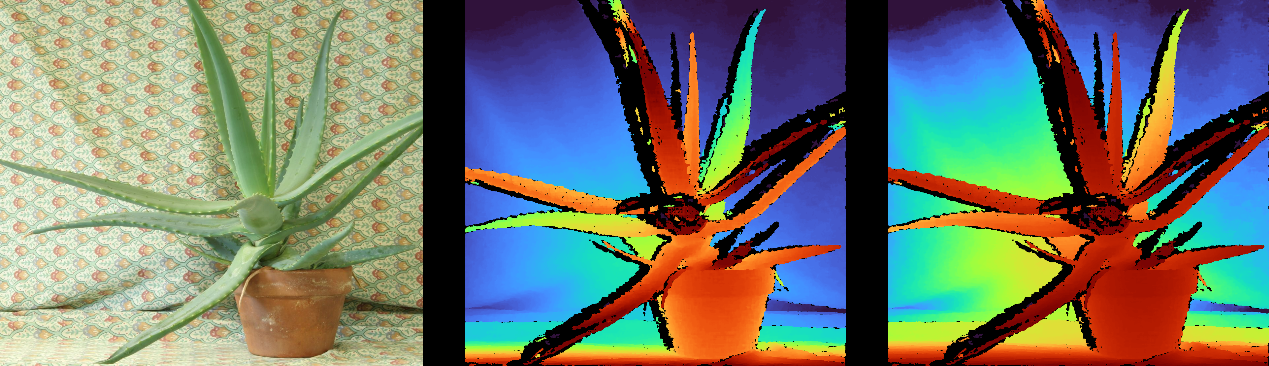
\includegraphics[width=\textwidth]{../results/stereo_result_panel.png}
\caption{Left image, disparity visualization, and relative-depth visualization.}
\end{figure}

\begin{figure}[H]
\centering
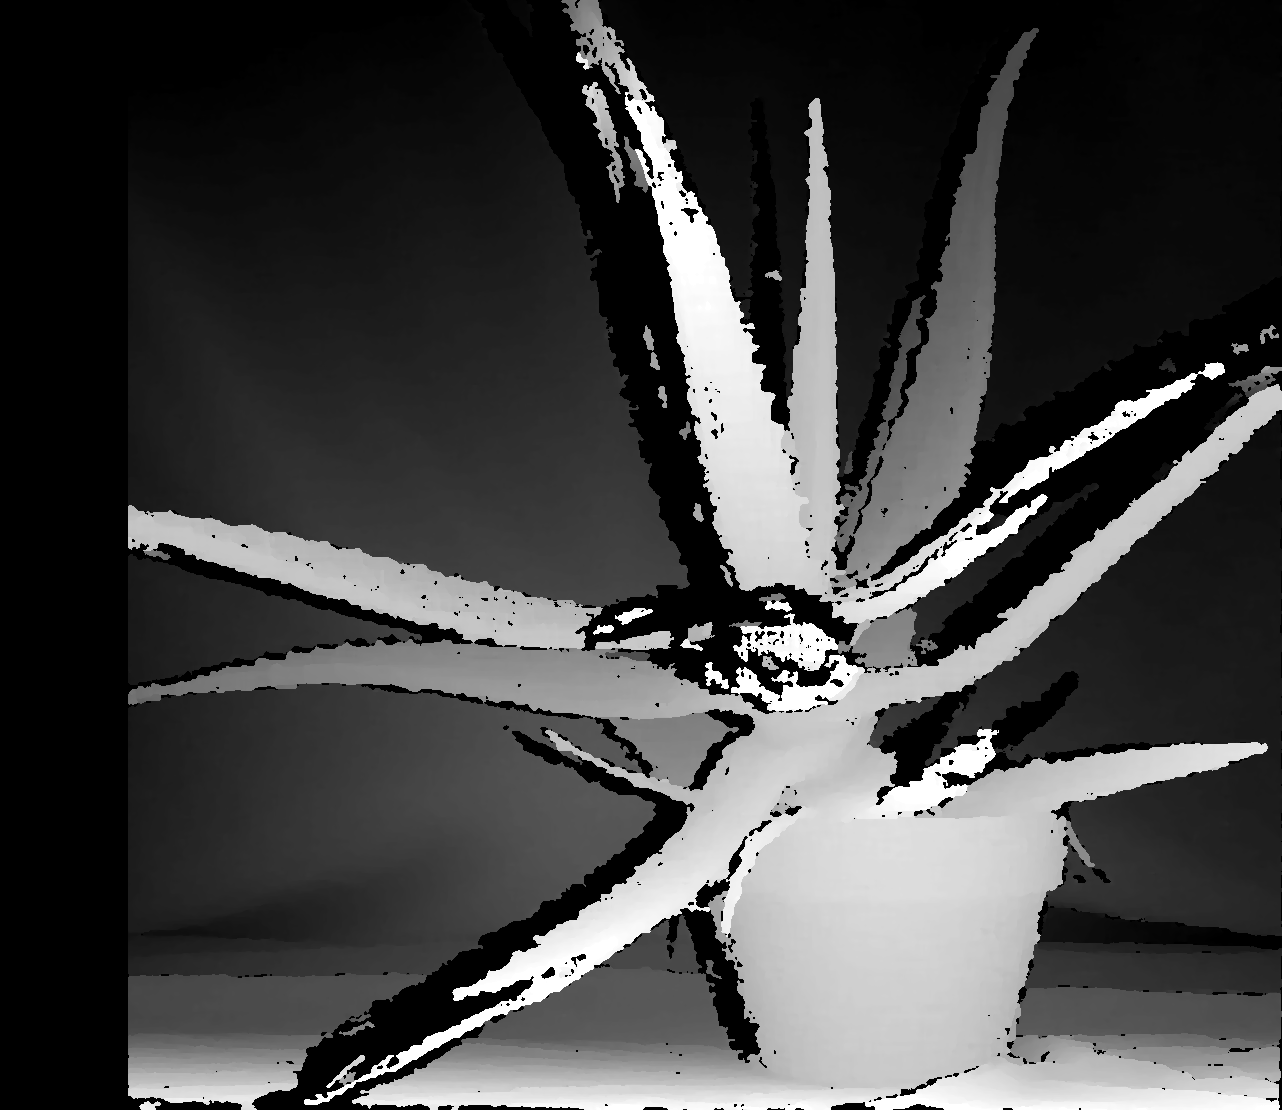
\includegraphics[width=0.68\textwidth]{../results/disparity_gray.png}
\caption{Normalized grayscale disparity map.}
\end{figure}

\section{Analysis and Discussion}
The plant leaves and flowerpot are estimated as closer than the patterned background because their disparities are larger. These regions have clear boundaries and rich texture, which supports reliable correspondence matching. The background has smaller disparity and appears in a different colour range.

Black regions occur where matching is unreliable, especially at occlusion boundaries, narrow leaf edges, and weakly textured areas. A pixel visible in one camera may be hidden in the other, so a valid correspondence is not always available. Repeated patterns can also create ambiguous matches.

A calibrated stereo camera would enable metric depth using focal length and baseline. Further improvement would include camera calibration, stereo rectification, and parameter tuning for the particular scene. This result is appropriate for comparing relative distance in the image pair, but not for reporting physical distance.

\section{Conclusion}
This experiment successfully implemented OpenCV-based stereo depth estimation with the official aloe stereo data. StereoSGBM produced a valid disparity ratio of 78.07\%, and the program exported disparity images, a relative-depth image, raw disparity data, and a comparison panel. The result demonstrates the inverse relationship between disparity and scene depth.

\section{Submission Record}
\begin{tabular}{p{4cm}p{9cm}}
\rowcolor{labgreen}\color{white}\bfseries Item & \color{white}\bfseries Record \\
\rowcolor{lightgreen}GitHub Repository & \url{https://github.com/Eva122205/opencv-stereo-depth} \\
Program Commit & \texttt{bb82872} -- Add StereoSGBM stereo depth estimation program \\
Results Commit & \texttt{739245f} -- Add stereo disparity and relative depth results \\
Report Commit & \texttt{4815395} -- Add stereo depth estimation lab report \\
\end{tabular}

\section{References}
\begin{enumerate}
\item OpenCV Documentation. StereoSGBM Class Reference.
\item OpenCV Sample Data Repository. \texttt{aloeL.jpg} and \texttt{aloeR.jpg} stereo pair.
\item H. Hirschmuller. Stereo Processing by Semiglobal Matching and Mutual Information. IEEE TPAMI, 2008.
\end{enumerate}

\end{document}
